\providecommand{\main}{..}
\documentclass[\main/main.tex]{subfiles}

\begin{document}
\graphicspath{{img/}{06_result/img/}}

\chapter{Result}

\section{Whole system overview}
\begin{figure}[H]
    \centering
    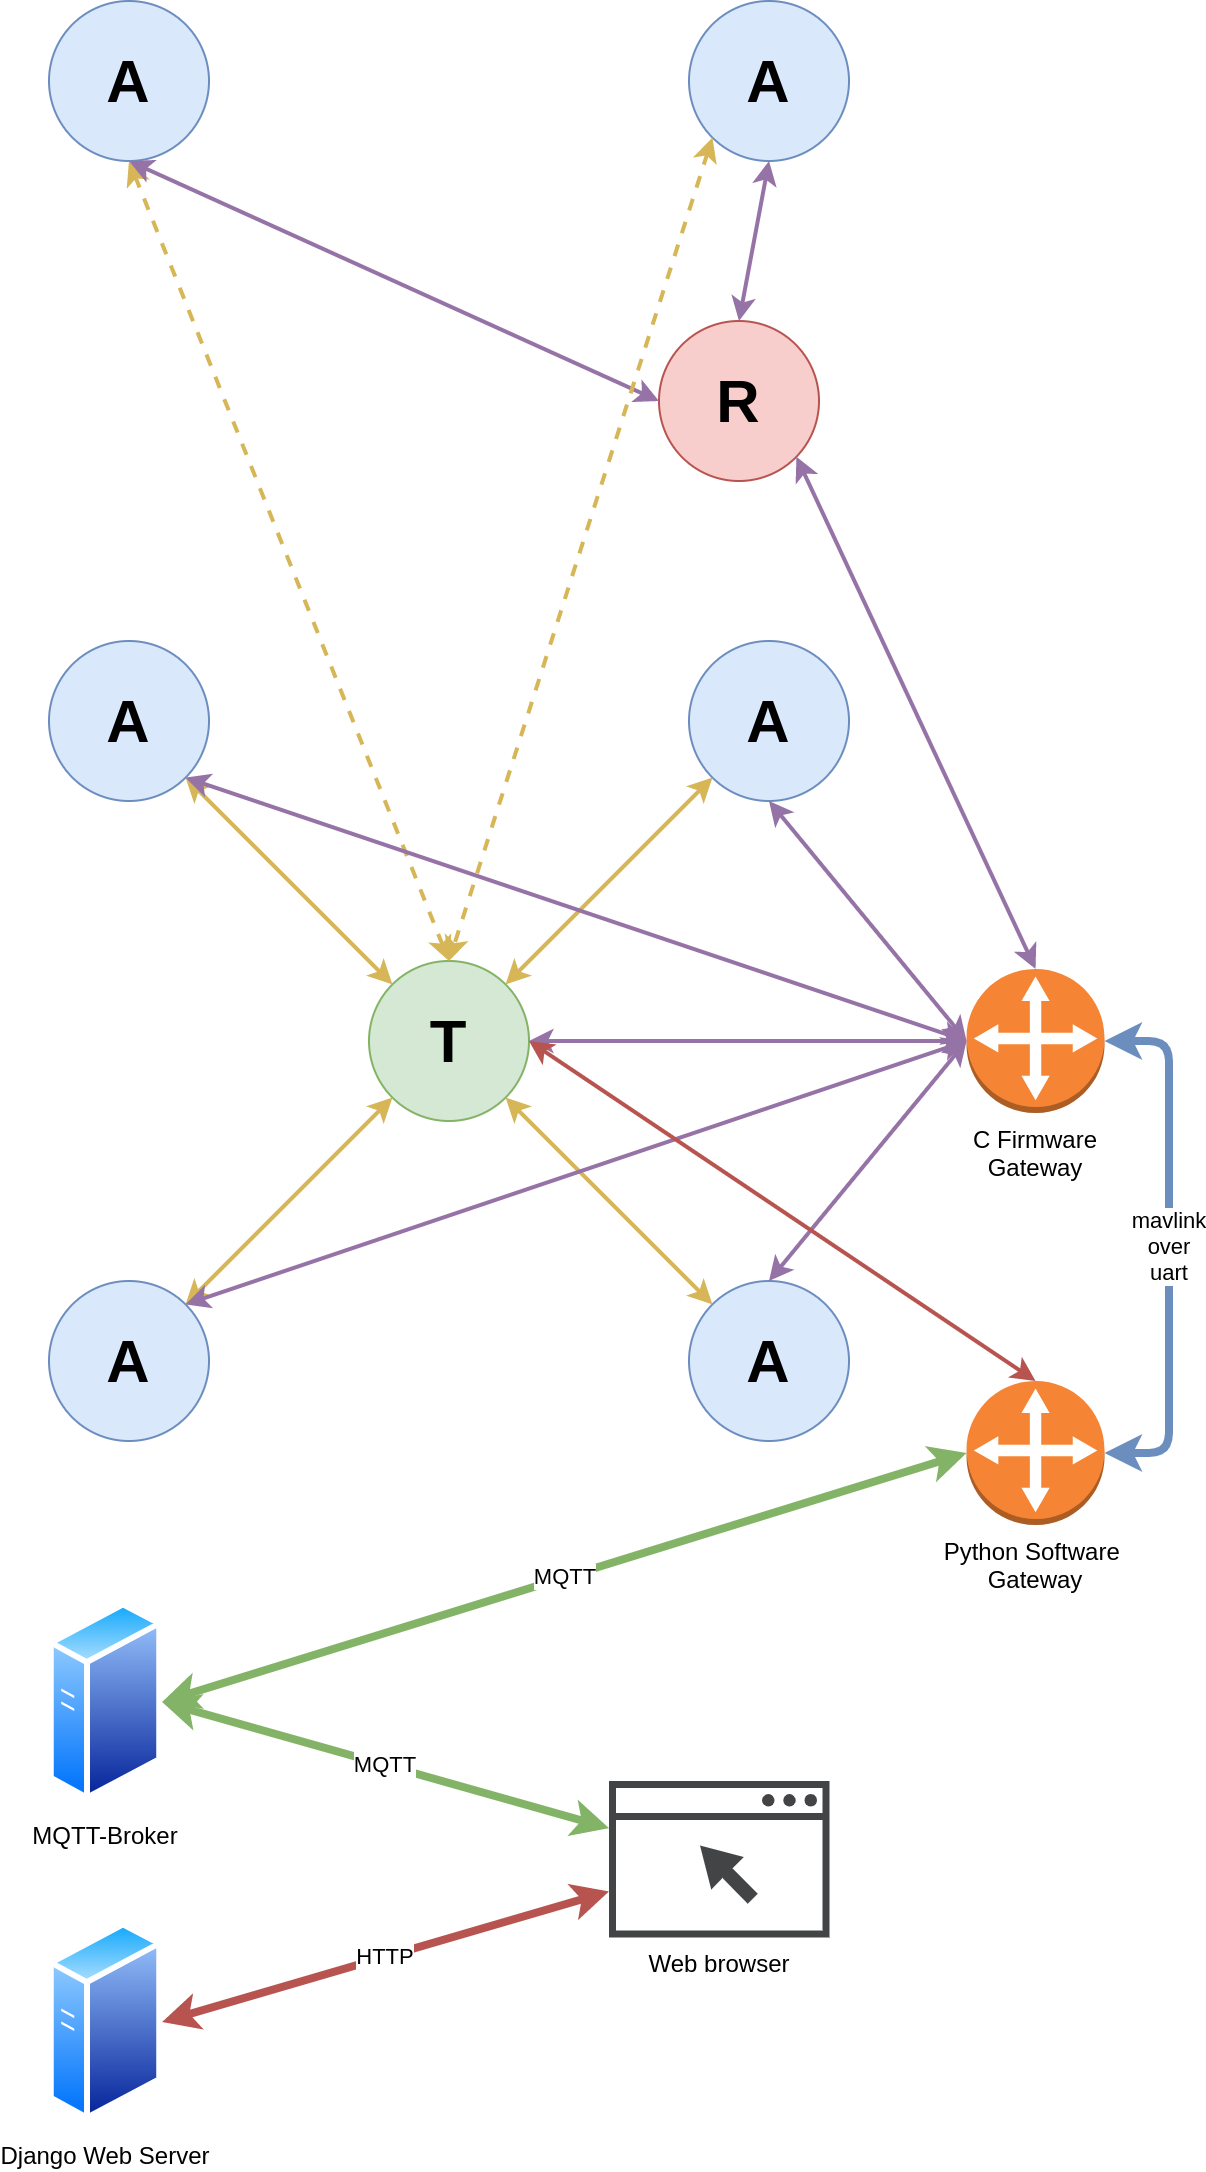
\includegraphics[width=0.45\textwidth]{system_overview.png}
    \caption{Whole system overview}
    \label{fig:system_overview}
\end{figure}

\section{CCP}

\section{TDMA}

\section{Ranging}

\section{BLE mesh}

\section{Localization}

Error formula:
\begin{equation}
    e_{RMS} = \sqrt{\frac{1}{n} \sum_{k=1}^{n} ((x_k-x_{kg})^2 + (y_k-y_{kg})^2)}
    \label{eqn:root_mean_square}
\end{equation}

\subsubsection*{Vendor demo}
\begin{table}[ht]
    \centering
    \begin{tabular}{|c|>{\centering\arraybackslash}p{2cm}|>{\centering\arraybackslash}p{2cm}|>{\centering\arraybackslash}p{2cm}|}
    \hline
    \backslashbox{y(m)}{x(m)}  &  3 & 7 & 10 \\ \hline
    0 &  0.2 &  0.28 &  0.25  \\ \hline
    2 &  0.14 &  0.13 &  0.18  \\ \hline
    4 &  0.22 &  0.19 &  0.27  \\ \hline
    \end{tabular}
    \caption{RMS error}
    \label{table:rms_error}
\end{table}

\begin{figure}[ht]
    \begin{minipage}[t]{\textwidth}       
        \centering
        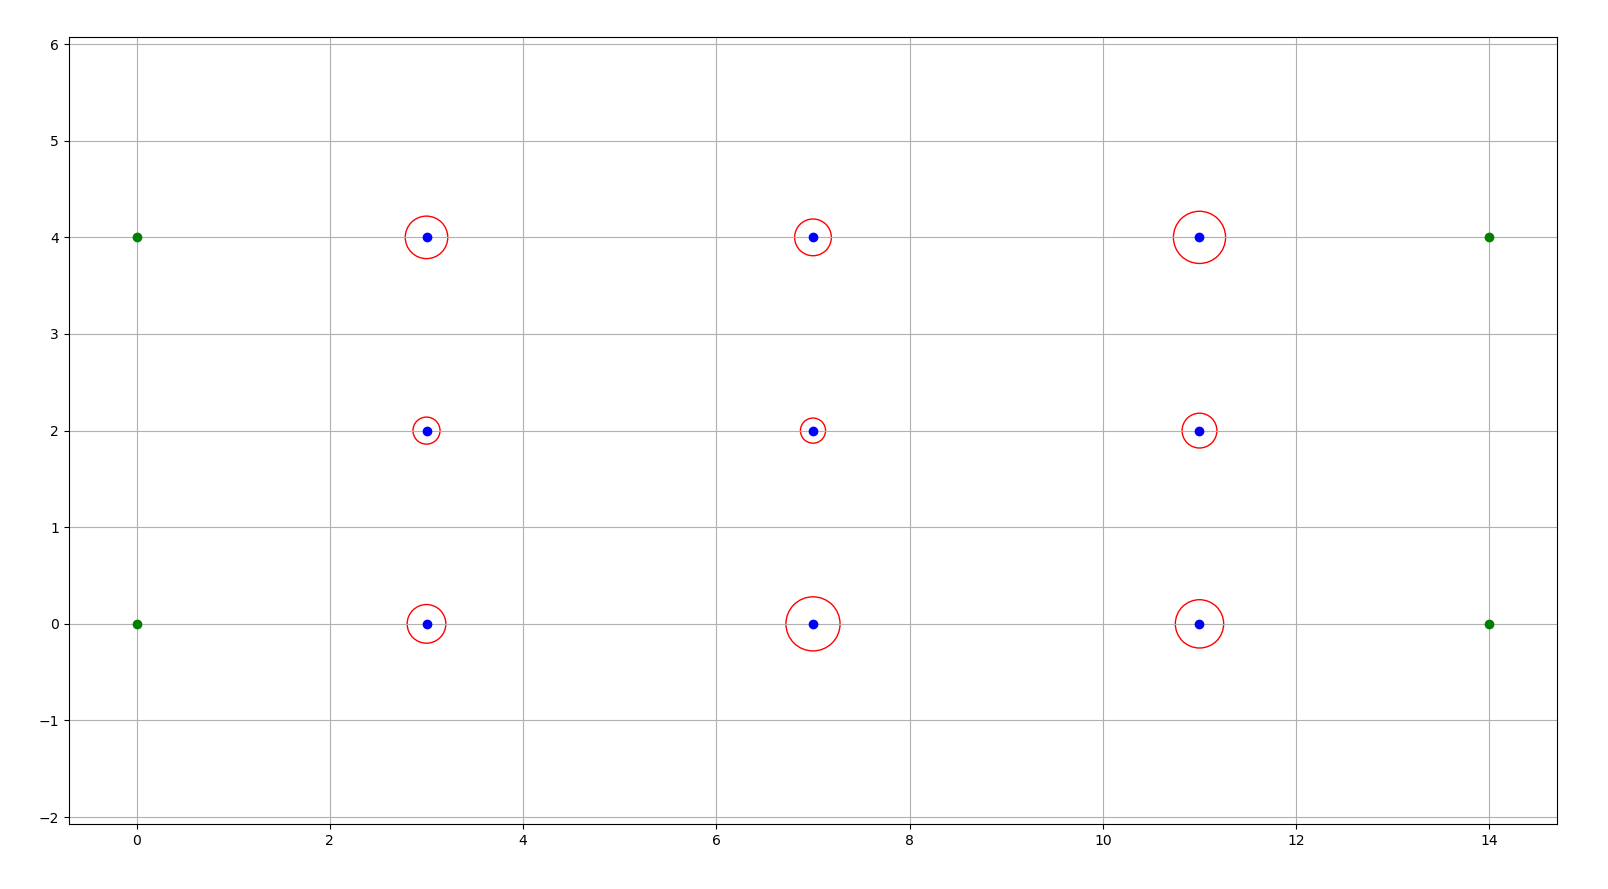
\includegraphics[width=0.7\textwidth]{rms_error}
    \end{minipage}
    \caption{Error map}
    \label{fig:rms_error}
\end{figure}

\subsubsection*{One cell localization}

\subsubsection*{Multi-cell localization}

\end{document}